% Created 2020-12-27 Sun 23:59
% Intended LaTeX compiler: pdflatex
\documentclass[sigconf,natbib,screen=true,review=true,anonymous]{acmart}

% We'll get the submission number fro the submission system
\acmSubmissionID{848}

% !TEX root = ./main.tex

% list your packages
\usepackage[utf8]{inputenc}
\usepackage[T1]{fontenc}
\usepackage{graphicx}
\usepackage{grffile}
\usepackage{longtable}
\usepackage{wrapfig}
\usepackage{rotating}
\usepackage[normalem]{ulem}
%\usepackage{amsmath}
\usepackage{textcomp}
%\usepackage{amssymb}
\usepackage{capt-of}
\usepackage{hyperref}
%\usepackage{minted}

\usepackage{algorithmic}
\usepackage{graphicx}
\usepackage{xcolor}
\usepackage{multirow} 
\usepackage{xcolor}
\usepackage[ruled,linesnumbered,boxed]{algorithm2e}
\usepackage[inline]{enumitem}
\usepackage{booktabs}
\usepackage[skip=0pt]{caption}
\usepackage{acronym}
\usepackage{url}
% \usepackage{graphicx}
% \usepackage{adjustbox}

\usepackage{xcolor}

%\usepackage{amsmath}
\usepackage{dsfont}
\usepackage{color}

% !TEX root = ./main.tex

% list your definitions
\newcommand{\mdr}[1]{\textcolor{orange}{\textbf{[#1]}}}
\newcommand{\daan}[1]{\textcolor{teal}{\textbf{[DO: #1]}}}
\newcommand{\mvm}[1]{\textcolor{blue}{\textbf{[MvM: #1]}}}
\newcommand{\hvk}[1]{\textcolor{pink}{\textbf{[HVK: #1]}}}

\newcommand\todo[1]{\textcolor{red}{TODO : #1}}
\newcommand\doubt[1]{\textcolor{orange}{DOUBT : #1}}
% \newcommand\todo[1]{} % uncomment to hide comments
% \newcommand\doubt[1]{} % uncomment to hide comments

\hypersetup{
 pdfauthor={Gabriel Bénédict},
 pdftitle={},
 pdfkeywords={},
 pdfsubject={},
 pdfcreator={Emacs 26.1 (Org mode 9.1.14)},
 pdflang={English}}

% !TEX root = ./main.tex

\author{Gabriel B\'en\'edict}
\affiliation{
\institution{RTL \& University of Amsterdam} 
\city{Amsterdam}
\country{The Netherlands}
}
\email{something}

\author{Daan Odijk}
\affiliation{
\institution{RTL} 
\city{Amsterdam}
\country{The Netherlands}
}
\email{something}

\author{Maarten de Rijke}
\affiliation{
\instutute{University of Amsterdam \& Ahold Delhaize}
\city{Amsterdam}
\country{The Netherlands}
}
\email{m.derijke@uva.nl}

% !TEX root =  ./main.tex 

\copyrightyear{2021}
\acmYear{2021}
\setcopyright{rightsretained}
\acmConference[SIGIR '21]{Proceedings of the 44th International ACM SIGIR Conference on Research and Development in Information Retrieval}{July 11-15, 2021}{Montr{\'{e}}al, Canada}
\acmBooktitle{Proceedings of the 44th International ACM SIGIR Conference on Research and Development in Information Retrieval (SIGIR '21), July 11-15, 2021, Montr{\'{e}}al, Canada}
\acmPrice{}
\settopmatter{printfolios=false}

\begin{CCSXML}
<ccs2012>
   <concept>
       <concept_id>10002951.10003317.10003347.10003356</concept_id>
       <concept_desc>Information systems~Clustering and classification</concept_desc>
       <concept_significance>500</concept_significance>
       </concept>
   <concept>
       <concept_id>10002951.10003317.10003318.10003321</concept_id>
       <concept_desc>Information systems~Content analysis and feature selection</concept_desc>
       <concept_significance>300</concept_significance>
       </concept>
 </ccs2012>
\end{CCSXML}

\ccsdesc[500]{Information systems~Clustering and classification}
\ccsdesc[300]{Information systems~Content analysis and feature selection}

\keywords{Content analysis; Classification; Multilabel classification; Custom loss functions}


\begin{document}

\title{SIMPUL: A Loss Framework to Learn Abstract Labels from Abstract Representations: Single-Instance Multiclass Multilabel Prediction with Unknown Label Count}

\begin{abstract}
Multilabel classification is a common task when learning from text, image, or sound. However, few optimization frameworks are tailored towards learning multiple abstract descriptors of an entire text, image, or sound. We present this problem as SIMPUL. \hvk{it is a bit confusing to me here that SIMPUL is presented as a problem, but as a framework in the title} Current solutions typically reframe the SIMPUL problem as a multiclass problem. This allows for the use of variations of cross-entropy or multinomial logit losses. When the number of ground-truth labels varies over each example, these losses produce unit-interval results that require a sophisticated thresholding regime (at training or at inference time) to predict both label prediction propensity and label count. As a solution to SIMPUL, we present \emph{sigmoidF1}: a decomposable surrogate F1 score that introduces smooth thresholding. The proposed method yields higher F1 metrics on several datasets of different modes. This shows that higher level abstractions in the embedding space can be directly predictive of abstract labels in the output space. The code is available at (https://anonymous.4open.science).
\todo{SIMPUL as a general confusion-metric-as-a-loss framework }



% \begin{itemize}
% \item \mdr{one sentence context}
% \item \mdr{one sentence problem statement}
% \item \mdr{one sentence what's wrong with current solutions}
% \item \mdr{one sentence our proposal}
% \item \mdr{one sentence the results achieved with our proposal}
% \item \mdr{one sentence why this matters}
% \end{itemize}
\end{abstract}

\keywords{Content analysis; Classification; Multiclass; Multilabel; Custom Loss \mdr{Keyword}}


\maketitle

\acresetall

% !TEX root = ../main.tex

\section{introduction}
\label{sec:org662677c}

As neural network models are able to learn increasingly more abstract representations via deeper networks, representation learning and self-supervision~\citep[see, e.g.,][]{XX,YYY,ZZZ}, it is reasonable to expect that they also get better at predicting more abstract labels. 
Beyond identifying object types~\mdr{REF}, performing face recognition~\mdr{REF}, \mdr{doing what with} expressions~\mdr{REF}, neural networks should soon be able to predict genres/categories of text, image and sound at high levels of accuracy. 
Towards this goal, there is a significant volume of recent work on building neural networks with high-level of understanding in the embedding space~\mdr{REF}.
However, there seems to be limited research on developing loss functions that are adapted for these higher level concepts in the output space.

\mdr{Briefly and concretely describe the abstract labeling task that we are interested in.}

To situate the specific problem that we tackle in this paper, it is helpful to consider Figure~\ref{fig:tree} so as to disambiguate our terminology. 
Figure~\ref{fig:tree} shows \mdr{what}.
There seems to exist a consensus over the terms \emph{multiclass} and \emph{multilabel learning}, meaning mutually exclusive and mutually inclusive labels, respectively \todo{source}. 
Multilabel learning can therefore be seen as a subdomain of multiclass learning, where more than one class can be true for the same example. 
Within multilabel training, we introduce the distinction between multi-instance multilabel~\citep[e.g.,][]{multiInstance}) and uni-instance multilabel. 
\mdr{vague: Multi-instance multilabel classification refers to tasks where elements within each example can be singled-out and assigned one or more labels; examples include objects \mdr{not a task} in an image or tokens in a text.}
Uni-stance multilabel classification is \mdr{define it}.
\begin{itemize}
\item \mdr{Now explain that the task introduced in the second paragraph is an instance of uni-instance multilabel classification.}
\item \mdr{Now make the distinction between fixed label counts and varying label counts}
\item \mdr{Little work has been done on the uni-instance, ML MC prediction with a varying number of classes}
\item \mdr{Identify the shortcomings o prior work on the task that we care about}
\end{itemize}

\begin{figure}[t]
\centering
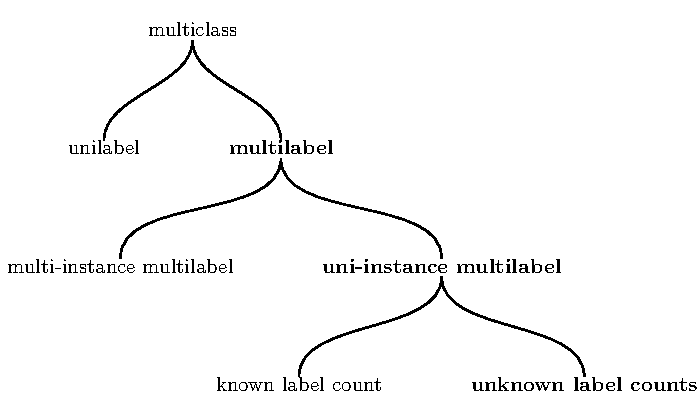
\includegraphics[width=.9\linewidth]{./tree/Tree.pdf}
\caption{\label{fig:tree}
Clarifying ``multiclass'' classification problems.}
\end{figure}

\mdr{Now we have a paragraph in which you clearly describe your proposed line of attack}

\mdr{Now we have a paragraph that explains the results that we have obtained with our proposed approach}

\mdr{Now we have a paragraph with our main contributions:}
\begin{itemize}[leftmargin=*]
\item \mdr{Contribution 1}
\item \mdr{Contribution 2}
\item \mdr{Contribution 3}
\end{itemize}

\mdr{The remainder of the paper is organized as follows. Expand.}

\vspace*{3cm}
\mdr{Move all of the content to other sections, e.g., to background section or to related work. Also, try to avoid the meandering narrative that touches on many points but sometimes forgets to make explicit what its main point is.}

In this paper we focus on uni-instance multilabel training (sparse occurences of the term holistic can be found in the literature to describe this phenomenon for image \cite{holisticImageDescriptors,holisticLungs} and a recent video dataset \cite{holisticVideoData} \todo{read these}), more specifically with varying label counts. To the best of our knowledge, there are few existing representatives of that type of labelling task in the literature. \todo{cite more milestone examples for each category.} \todo{delta with hierarchical label learning}

\mdr{Too talkative, too many diverse angles. Make sure that there is a clear point that you are making:}
Although multilabel binary prediction (commonly referring to mutually inclusive labels) is a task thoroughly covered in existing literature, there does not seem to exist a framework that deals with different amounts of positive labels in the groundtruth. For example, a scientific journal can be tagged as \emph{machine learning} and \emph{economics}, or a movie can be tagged as \emph{romance} and \emph{comedy}. These instances might as well be assigned only one tag in the groundtruth, or many more within the possible tags (classes).


The particularity of tasks like scientific paper tagging or movie genre classification is that it remains unclear what elements in an image/video or text can be singled out as predictive of a particular tag/genre. Rather, a complex interaction between these elements in the feature space steer the predictions. For example, the sole mention of the term "machine learning" in a paper should not be a sufficient condition to tag it as such. Instead, one could expect from the publisher to get acquainted with the paper enough to determine wether the research is a worthwhile contribution or application of \emph{machine learning} to deserve the tag. This involves thorough understanding of the proposed method and background knowledge on state-of-the-art methods. An analogous argument can be made for movie genre classification for movie posters.

However, if elements in an image/text can be singled out as predictive of a single tag, the problem reverts back to predicting with the a priori knowledge of the existence of only one true label (i.e. multi-instance multilabel learning).  The reason for distanciating singling-out from uni-instance labels, is that it has been shown that as soon as singling-out is possible, models that work on instances are more accurate \todo{rewrite this paragraph and sources}. The singled-out elements can be subsets of the original feature space (typically in object detection like with the COCO dataset  \cite{COCO} or the Amazon Rainforest Dataset\footnote{Available at \url{https://www.kaggle.com/c/planet-understanding-the-amazon-from-space}} \todo{others}). Similarly, recent research has shown that the singled-out elements can be located in the abstract representations (embeddings) of the feature set and might individually predict a single true label (like GPT-3 \todo{source}) \todo{more examples}. This might also carry prospects of generalizability of the model \cite{generalization} \todo{elaborate}. 

But for now, in certain retrieval tasks such as scientific journal tagging, the effect of sub-entities (either expressions in the text or single features in the embedding space) on the prediction of each label remains hard to assess. Instead we propose uni-instance (sometimes referred to as holistic) multilabel learning for varying amount of labels, with a focus on custom loss functions.

To allow the use of existing diffentiable loss fonctions, previous research papers tend to reframe the problem into either (I) a multi-instance multiclass (as described above, with the COCO dataset as an example of isolation of features \cite{COCO}), (II) uni-instance multiclass prediction (III) uni-instance multilabel prediction with fixed label count (IV) uni-instance multilabel prediction with varying label count with post-training thresholding (V) redefine backpropagation for multilabel prediction \cite{multilabelBackprop} (VI) multitask learning \cite{multitaskLabel} (VII) custom loss function \cite{tencent}. This order reflects in ascending order how close modelling seem to fit the original task, which remains uni-instance multilabel learning with varying amounts of labels. \doubt{group them}

Common loss functions such as cross-entropy loss (for mutually inclusive labels) or multinomial logit loss (for mutually exclusive labels) deliver predictions on the unit interval. Thresholding the output to assess the performance of the model against the groundtruth can be done after training for (I), (II), (III) and (IV). \todo{give a very sound reason as to why we'd rather not do things post-training and rather at training-time}. Problem formulations (V), (VI) and (VII) suggest a solution at training time. We think that a custom loss function (VII) is the best alternative. \todo{explain why}

In a number of retrieval tasks, a model's out of sample accuracy is measured on metrics such as AUROC, F1 score, etc. These reflect an objective catered towards evaluating the model over an entire ranking. Due to to lack of differentiability, these metrics cannot be directly used as loss functions at training time (in-sample). A seminal study \cite{optimizableLosses} derived a general framework for deriving decomposable surrogates to some of these metrics. We propose our own decomposable F1 surrogate tailored for the problem at hand.

\mdr{This paragraph can probably be kept in the introduction}
We first propose a general mathematical formulation of uni-instance multilabel learning for varying amount of groundtruth labels. The generalization encompasses different levels of complexity, from the classical cross-entropy loss up to the proposed loss function. \emph{sigmoidF1} is a F1 score surrogate which allows to optimize for label prediction and count simultanuously in a single task and is robust to outliers. It delivers more precise predictions than the current state-of-the-art on several different metrics, accross text and image related tasks. \emph{sigmoidF1} and its adaptive \emph{SadF1} and Bayesian \emph{SBayesF1} counterparts are benchmarked against loss functions commonly used in multilabel learning and others tailored specifically to the uni-instance multilabel with varying number of labels setting.

%% !TEX root = ../main.tex

\section{Task Definition}

In this section, we use Figure~\ref{fig:tree} to further disambiguate the current method, by walking down its structure and explain why we avoid the left-leaning branches. We finish by showing how previous research focusing on problems down the tree tends to climb the tree back up to higher level of abstractions when looking for solutions.

Starting at the top of the tree, multiclass unilabel classification is often solved with common loss functions like cross entropy, mutinomial logit or focal loss. To the right, multiple labels can be assigned for the same example (e.g. movie genres, phenotypes). climbing down this time, multilabel tasks are often affiliated to image and text classification, where subsets of the original feature space can be singled out as predictive of a label (typically in object detection like with the COCO dataset  \cite{COCO} or the Amazon Rainforest Dataset\footnote{Available at \url{https://www.kaggle.com/c/planet-understanding-the-amazon-from-space}} \todo{others} \daan{a citation would be better here.}). Once elements are singled out, it is often trivial to allow each element to be only predictive of one label: the task often comes down to attributing a single label to an object or an expression. When it is technically possible to single out elements of an example that are predictive of a single label (or a lesser amount of labels), it is preferable to single-out rather than to predict given the entire image / text / audio~\cite{multiInstanceMultiLabel}.

In our setting, we deliberately deal with cases where it is not possible to single out elements. For example, expressions within a paper abstract, single notes within a song, or individual character stance within a movie poster can not be singled-out to be uniquely predictive of a single label. Rather, it is the interaction between the terms in the definition of the current study that could eventually classify this paper as a machine learning and information retrieval paper. Similarly, an actor holding a gun in a movie poster with otherwise jolly faces and background will probably not be an action/thriller movie, but rather a (dark) comedy. 

At the bottom of the tree, the situation where the number of labels $n_i$ to predict for each example is known a priori will deliberately be dodged. In that case, common information retrieval algorithms can retrieve ranks and thus $top_{n_i}$ predictions \todo{source}.
\daan{My feeling was that this was where we make the most significant contribution, in better distributing the loss over an unknown number of labels. If so, then this should be the gist of this section of text.}

We are left with the branch at the bottom right of the tree. Namely, we define the problem of single-instance multilabel learning for varying amount of labels.

Note that Figure~\ref{fig:tree} could be further divided into different branches starting from the bottom right corner. In particular, frameworks that study the relationships between labels like holistic label learning (as seen for image \cite{holisticImageDescriptors,holisticLungs} and video dataset \cite{holisticVideoData} \todo{read these}) and hierarchical label learning~\cite{activeLearningMultiLabel, HARAM} are left out of the picture, in order to focus on the general MSILUL formulation. \daan{MSILUL? Earlier acronym?}

We now briefly discuss the \emph{climbing-up} phenomenon described at the beginning of this section. To allow the use of existing differentiable loss fonctions, previous research papers tend to re-frame a problem at the bottom of the tree into models that learn for (I) multi-instance multiclass (as described above, with the COCO dataset as an example of isolation of features \cite{COCO}), (II) single-instance multiclass prediction \cite{multiclass} (III) single-instance multilabel prediction with fixed label count~\cite{threshForF1}. In other terms this relates to problem transformation, further detailed in the next section.

\daan{I am not very convinced by this section. I can see how the three helped shaped your thoughts, but let's discuss whether it helps sell the paper.}



% Similarly, recent research has shown that the singled-out elements can be located in the abstract representations (embeddings) of the feature set and might individually predict a single true label (like GPT-3 \todo{source}) \todo{more examples}. This might also carry prospects of generalizability of the model \cite{generalization} \todo{elaborate}.

% But for now, in certain retrieval tasks such as scientific journal tagging, the effect of sub-entities (either expressions in the text or single features in the embedding space) on the prediction of each label remains hard to assess. Instead we propose single-instance multilabel learning for varying amount of labels, with a focus on custom loss functions.







% In this section we provide a formal definition of the uni-instance multiclass multilabel problem with a varying number of labels on which we focus in this paper.
% \begin{itemize}
% \item Give a precise, formal definition of the problem 
% \item If appropriate, indicate formally fixed label counts vs.\ varying label counts 
% \item If appropriate, indicate formally uni-instance vs multi-instance
% \item Give three example instances of the problem (you could be inspired by the datasets that we use later in the paper)
% \end{itemize}
% !TEX root = ../main.tex

\section{Background}
\label{sec:org8c910ea}

In this section, we recall the background material needed to be able to introduce our proposed solution to the MSILUL problem.

Multilabel learning can be divided into two major fields: \emph{problem transformation} and \emph{algorithm adaptation} \cite{multilabelReview}. In the former case, multilabel classification is reframed as a binary, multiclass classification or label ranking problem. In the latter, one tries to adapt multiclass algorithms to the problem. The current endeavor focusses on \emph{algorithm adaptation}.


For the purpose of \emph{problem transformation}, we define \(\mathcal{L}_{\text {multiclass}}\), a class of loss functions that minimize predictions in relative terms. Binary cross-entropy, logit and their variants such as focal loss or hinge loss (deemed unstable \cite{focalLoss}) are common choices when it comes to multiclass prediction. Cross-entropy loss can be formulated as \(\mathcal{L}_{\text {CE}}=-\sum \log \left(p_{i}\right)\) . Note that minimizing binary cross-entropy is equivalent to maximizing for log-likelihood \cite[Section 4.3.4]{Bishop}. More generally, the \emph{problem transformation} formulation amounts to minimizing the loss on a class of neural networks, such that
%
\begin{equation}
\underset{\mathcal{L}_{\text {multiclass}}} {\min} \mathcal{F}\left(\cdot ; \Theta; \mathcal{L}_{\text {multiclass}} (\mathbf{y}, \hat{\mathbf{y}}) \right),
\end{equation}
%
In the context of \emph{algorithm adaptation}, where the number of positive labels in the groundtruth is unknown a priori, we aim to both obtain a propensity of each label being true and a prediction of the number of true labels: 
%
\begin{equation}
\underset{\mathcal{L}_{\text {multiclass}}, \mathcal{L}_{\text {count}}} {\min} \mathcal{F}\left(\cdot ; \Theta; \mathcal{L}_{\text {multiclass}} (\mathbf{y}, \hat{\mathbf{y}}) + \lambda \mathcal{L}_{\text {count}} (\mathbf{n}, \hat{\mathbf{n}})\right),
\end{equation}
%
where \(n_i = \sum_j \mathds{1}_{\mathbf{y_i^j} = 1}\) is the count of positive labels per example. We thus impose a constraint for the retrieval of label counts. For example, a cross-entropy loss surrogate would penalize for the number of wrongly predicted labels \(\mathcal{L}_{\text {CE+N}}= \mathcal{L}_{\text {CE}} + \lambda (\sum tp / \sum p)\), with \(t p=\sum_{i \in Y^{+}} \mathds{1}_{\mathbf{p_i} \geq b}\) and \(b\) a threshold to be defined. With its multitask framework (predict label prediction propensity and label count) \cite{multitaskLabel} corresponds to that type of infrastructure. \todo{tencent loss}.

The latter formulation is most straightfoward but suffers from higher parametrization and the lack of modelling of the interactions between label counts and label prediction. To mitigate these issues, we propose a unified loss formulation, namely
%
\begin{equation}
\underset{\mathcal{L}_{\text {multitag}}} {\min} \mathcal{F}\left(\cdot ; \Theta; \mathcal{L}_{\text {multitag}} (\mathbf{y}, \hat{\mathbf{y}}, \mathbf{n}, \hat{\mathbf{n}}) \right),
\end{equation}
%
Although predictions and counts explicitly appear in that formulation, \(\mathcal{L}_{\text {multitag}}\) can optimize for both metrics implicitely (see proposed \emph{sigmoidF1} below).



% (IV) uni-instance multilabel prediction with varying label count with post-training thresholding (V) redefine backpropagation for multilabel prediction \cite{multilabelBackprop} (VI) multitask learning \cite{multitaskLabel} (VII) custom loss function \cite{tencent}. This order reflects in ascending order how close modelling seem to fit the original task, which remains uni-instance multilabel learning with varying amounts of labels. \doubt{group them}


\todo{look at YOU ONLY TRAIN ONCE: LOSS-CONDITIONAL TRAINING OF DEEP NETWORKS}

\todo{cite stat learning}   \cite[p. 308-310]{statLearning}

\todo{show that I am between the two extremes of Pure multiclass with post thresholding and multiclass + penalty for num labels}
\todo{can I rewrite L CN + N into F1}

% * our contribution

% In order to verify our hypotheses, we use multilabel examples, where it is arguably hard to distinguish which elements is predictive of the label. For example, movie posters where the whole context is important and not just facial expressions, title font.

% !TEX root = ../main.tex

\section{Method}
\label{sec:orga8a42f5}

\mdr{In this section we introduce the Sigmoid F1 Loss. We proceed as follows.}

For a class of multilayer perceptron \(\mathcal{F}(\cdot ; \Theta): \mathcal{X} \rightarrow \mathcal{Y}\), we consider a special case, where \(\mathbf{x} = \{x_1, ..., x_n\}\). Each observation is attributed one or more classes out of a label set \(\mathbf{l} = \{l_1, ..., l_c\}\). Labels \(y_{i}^{j}\) are available for each observation \(i\) and class \(j\). 

For each observation \(i\), label class probabilities can be defined based on predictions as

\todo{check this formula}

\begin{equation}
\mathbf{p}_{i}=\left\{\begin{array}{ll}\hat{\mathbf{y}} & \text { if } y=1 \\ 1-\hat{\mathbf{y}} & \text { otherwise }\end{array}\right.
\end{equation}

Let \(tp\) and \(fp\) be number of true and false positives respectively. It is necessary to define a bound \(b\), at which a prediction is dichotomized:

\begin{equation}
\label{eq:conf}
 t p=\sum_{i \in Y^{+}} \mathds{1}_{\mathbf{p_i} \geq b} \quad f p=\sum_{i \in Y^{-}} \mathds{1}_{\mathbf{p_i} \geq b} \quad fn = \sum_{i \in Y^{+}} \mathds{1}_{\mathbf{p_i} < b}
\end{equation}

\(\mathds{1}_{\mathbf{p_i} \geq b}\), \(\mathds{1}_{\mathbf{p_i} < b}\) are thus the count of positive and negative predictions at threshold \(b\), 

We also define precision and recall

\begin{equation}
\begin{aligned} P &=\frac{t p}{t p+f p} \\ R &=\frac{t p}{t p+f n}=\frac{t p}{\left|Y^{+}\right|} \end{aligned}
\end{equation}

We can then define \(F_\beta\), which can be expressed as the effectiveness of retrieval with respect to a user who attaches \(\beta\) times as much importance to recall than precision \cite{informationRetrieval}.

\doubt{maybe ignore $F_\beta$ and only mention $F_1$}

\begin{equation}
F_{\beta}=\left(1+\beta^{2}\right) \frac{P \cdot R}{\beta^{2} P+R}
\end{equation}

Or equivalently:

\begin{equation}
\begin{aligned} F_{\beta} &=\left(1+\beta^{2}\right) \frac{t p}{\left(1+\beta^{2}\right) t p+\beta^{2} f n+f p} \\ &=\left(1+\beta^{2}\right) \frac{t p}{\beta^{2}|Y+|+t p+f p} \end{aligned}
\end{equation}

Given the presence of the step indicator function \(\sum \mathds{1}_{\mathbf{p_i} \geq b}\), \(F_\beta\) is not differentiable for gradient based methods. One way of surpassing that problem is to use a smooth surrogate.

\subsection{soft F1 score}
\label{sec:org3ca83ef}

It is possible define a \emph{soft F1} score \cite{softF1} \doubt{can we cite a Medium post?} with smooth confusion matrix entries (i.e. \(tp\), \(fp\) and \(fn\) are not natural numbers anymore):

$$
\overline{tp}=\sum \hat{\mathbf{y}} \odot \mathbf{y} \quad \overline{fp} = \sum \hat{\mathbf{y}} \odot (\mathbf{1}- \mathbf{y}) \quad \overline{fn} = \sum (\mathbf{1} - \hat{\mathbf{y}}) \odot \mathbf{y}
$$

\begin{equation}
\mathcal{L}_{\text {softF1}}= \frac{\overline{tp}}{2 \overline{tp}+ \overline{fn}+ \overline{fp}}
\end{equation}

\(tp\), \(fp\) and \(fn\) are now replaced by rough surrogates, this method has the advantage of 

% /softF1/ is
% $$\mathcal{L}_{\text {Pred}}=\sum_{i, j}\left(\mathbf{y}_{i j}-\hat{\mathbf{y}}_{i j}\right)^{2}$$

\subsection{sigmoidF1 score}
\label{sec:orgc5d29d7}

We define \emph{sigmoidF1}, inspired by the \emph{Maximum F1-score criterion} for automatic mispronunciation detection \cite{sigmoid}. Whereas a sigmoid function \(S(u)\)

\begin{equation}
S(u; \beta, \eta)=\frac{1}{1+\exp (-\beta (u + \eta))},
\end{equation}

with \(\beta\) and \(\eta\) tunable parameters for slope and offset respectively. Higher \(\beta\) results in steeper slope at the center of the sigmoid and thus more stringent thresholding. At its extreme, \(lim_{\beta\to\infty} S(u; \beta, \eta)\) corresponds to the step function used in Equation \ref{eq:conf}. with \(S(u)\), the confusion matrix entries then become

\begin{equation}\label{eq:sigmoidF1}
\widetilde{tp}=\sum S(\hat{\mathbf{y}}) \odot \mathbf{y} \quad\widetilde{fp}= \sum S(\hat{\mathbf{y}}) \odot (\mathbf{1} - \mathbf{y}) \quad \widetilde{f n}= \sum (\mathbf{1} - S(\hat{\mathbf{y}})) \odot \mathbf{y}
\end{equation}

And thus

\begin{equation}
\mathcal{L}_{\text {sigmoidF1}}= \frac{\widetilde{tp}}{2 \widetilde{tp}+ \widetilde{fn}+ \widetilde{fp}}
\end{equation}

\doubt{mention smooth hinge loss} \cite{smoothHinge}

For \emph{sigmoidF1} \(\beta\) and \(\eta\) are tuned globally as hyperparameters. \emph{SAdF1} (Sigmoid Adaptive F1), is an alternative where \(\beta\) is first set to a relatively low value and increased after each epoch. This way, a loose threshold first allows Stochastic Gradient Descent (SGD) to broadly scan the parameter space accross several local minima, before narrowing parameter search down to a promissing region (similarily to adaptive learning rates).

\emph{SBayesF1} (sigmoid Bayes F1) replaces point estimates for \(\beta\) and \(\eta\) with posterior distribution estimates. 

\begin{equation}
\dot{S}(u_i) = \frac{1}{1+\exp (-\beta_i (u_i + \eta_i))}
\end{equation}

$$ \beta_i \sim N(0, \sigma^{2}_{\beta}) $$

$$ \eta_i \sim N(0, \sigma^{2}_{\eta}) $$

\(\beta_i\) and \(\eta_i\) are estimated with MCMC at training time of the neural network. They are therefore implicitely allowed to vary across examples. The \(\dot{tp}\), \(\dot{fp}\) and \(\dot{fn}\) surrogates can be formulated similarly to Equation \ref{eq:sigmoidF1}. We thus have

\begin{equation}
\mathcal{L}_{\text {SBayesF1}}= \frac{\dot{tp}}{2 \dot{tp}+ \dot{fn}+ \dot{fp}}
\end{equation}


% $\doublewidetilde{tp}$
% https://tex.stackexchange.com/questions/321231/double-widetilde
% doesn't work

\todo{try SadF1 and SBayesF1 in practice}


\subsection{Robustness}
\label{sec:org6c7c3d0}


Similarly to the focal loss \cite{focalLoss}, sigmoidF1 loss deals with class imbalance, robustness to outliers.

\todo{statistical robustness assessment}



\subsection{Evaluation Metrics}
\label{sec:org23c8447}

\mdr{Should this be here or in the Exp Setup section?}

The metrics described below are a result of a survey of different common practices for measuring accuracy of multilabel prediction. When true positives and false positives are used, recall that \(t p=\sum_{i \in Y^{+}} \mathds{1}_{\mathbf{p_i} \geq b}\) and \(f p=\sum_{i \in Y^{-}} \mathds{1}_{\mathbf{p_i} \geq b}\), and thus a threshold \(b\) must be set. When \(b = 0.5\), as is commonly done \todo{add source}, a risk remains that a lot of examples remain without predictions.

Extending \(F_1\) to multi-class binary classification amounts to deciding wether to un/pool classes.
In a first pooled iteration, micro \(F_1\) [SOURCE HERE] equates to creating a single 2x2 confusion matrix for all classes:
$$F_1^{micro} = \frac{\sum tp_c}{2 \sum tp_c + \sum fn_c + \sum fp_c} \quad for \quad c \in C$$

Macro \(F_1\) \cite{threshForF1} amounts to creating one confusion matrix per class or unpooling:

$$F_1^{macro} = \frac{1}{c} \sum_{j=1}^c F_1$$

\doubt{Do we need to justify optimizing for an F1 surrogate at training time and to then use F1 itself as a metric?}
% $$F_1^{macro} = \frac{\sum tp_c}{2 \sum tp_c + \sum fn_c + \sum fp_c} \quad for \quad c \in C$$

Weighted macro \(F_1\) \todo{find source} is similar but includes weighing to account for class imbalance, i.e. weighing each class by the number of groundtruth positives.
\begin{equation}
F_1^{weighted} = \frac{1}{c} \sum_{j=1}^c n_j F_1 \text{ where } n_j = \sum_i \mathds{1}_{\mathbf{y_i^j} = 1}.
\end{equation}

% $$F_1^{weighted} = \frac{\sum tp_c}{2 \sum tp_c + \sum fn_c + \sum fp_c} \quad for \quad c \in C$$

Accuracy is the overall fraction of correctly predicted labels \cite{threshForF1}:

$$
A c c=\frac{t p+t n}{t p+t n+f p+f n}
$$

Note that accuracy assigns equal cost to false positives and false negatives. This is particularly problematic in an unbalanced setup like here.

% - 'samples':
% Calculate metrics for each instance, and find their average (only meaningful for multilabel classification where this differs from accuracy_score).

% $$F_1^{micro} = \frac{\sum tp_c}{2 \sum tp_c + \sum fn_c + \sum fp_c} \quad for \quad c \in C$$

More variations scores exist in the literature, such as hamming loss~\cite{hammingLoss} (the fraction of incorrectly predicted labels), hamming score.q


\todo{compare to this:} \cite{lossComp}

\todo{Hamming Loss}
\todo{Precision@K, Recall@K, NDCG@K}
\todo{MLTSVM loss and the three-way loss inspired by it} \cite{MLTSVM} and \cite{MLTSVMThreeway}

\todo{explain batch size mathematically for F1 surrogate losses}
% !TEX root = ../main.tex

\section{Experimental Setup}
\label{sec:orgb44ba25}

sigmoidF1 is tested across different modalities, namely image, video, sound and text, with a focus on text: the most comparable research was on text data.

% \doubt{optional paragraph}
% In light of the problem definition leading to the sigmoidF1 framework in the introduction and in order to clearly delimit the proposed method, following are a few datasets that are not suitable for the task.


Among the three datasets used for benchmarking ML-NET \cite{multitaskLabel}, a cancer hallmark dataset is of multi-instance multilabel nature \cite{cancerHallmarks}\footnote{Available at \url{https://www.cl.cam.ac.uk/&sim;sb895/HoC.html}}: the research clearly describe a process of annotating several expressions within paper abstracts. The remaining two datasets for chemical exposure \cite{chemExposure}\footnote{Available at \url{https://figshare.com/articles/Corpus_and_Software/4668229}} and diagnosis codes assigment \cite{diagnosisCode}, \footnote{Available at \url{https://physionet.org/works/ICD9CodingofDischargeSummaries}} seem to fit to the entity wide multilabel definition but have a strong hierarchical nature. Although slightly out-of-scope, the three datasets above will be used for benchmarking, since they were used to test ML-NET, which is the state-of-the-art in \emph{algorithm adaptation} for text to the best of our knowledge.

For a broader scope in learning for text data, we also use the newly created \emph{Arxiv dataset}\footnote{Available at \url{https://www.kaggle.com/Cornell-University/arxiv}} with data on abstracts of 1.7 million open source articles and their categories (suitably mutually inclusive and of varying count per example).

In the vision domain, a dataset of movie posters\footnote{Labels available at https://tinyurl.com/y7ydyedu and prescraped images from IMDB at https://tinyurl.com/y7lfpvlx} and their genre is used. Similarly, labels are mutually inclusive and of varying count per example. It is arguable that is hard to single out elements in the image of a poster that define the genre of a movie. Rather it might be a combination of the title font, the background image, the presence of actors and specific objects such as cars, weapons etc. 




\todo{I removed all jpg's that are empty in the prescraped data. I could try to scrape the posters myself to see if I get more}

Another recently created dataset was made available for \emph{Large Scale Holistic Video Understanding} \cite{holisticVideoData} \footnote{Available at https://github.com/holistic-video-understanding/HVU-Dataset}, as defined in the introduction.

% Cancer can be described according to its complexity with different principles, named hallmarks cite:cancerHallmarks. A corpus of 1580 PubMed abstracts are manually annotated for 10 hallmarks. This is a multi-instance labelling task and will therefore not be used here.

% [[./images/cancerHallmarksAnnotation.jpg]]

% - Multilabel classification for text cite:toxicComments

% - Scenery dataset for images cite:dataScenery.

\todo{this is an ambitious number of datasets. Add longer description of each dataset, depending on which ones I keep: sample size, number of classes etc. see utils here: https://github.com/ashrefm/multi-label-soft-f1}

\doubt{cite Kaggle datasets formally instead of using links: https://www.kaggle.com/data/46091}

\doubt{add a music genre classification dataset, for which Vincent Koops at RTL could help train}



% !TEX root = ../main.tex

\section{Experimental Results}
\label{sec:orgc23a664}

varying b in the sigmoid function as if it is an adaptive learning rate \todo{actually try it out}.

one b per class

if we consider \(b\) and \(c\) to be probabilistic, we can then use tensorflow probability to assess their distribution

the batch size has to be relatively large (i.c. 256), in order for meaningful F1 surrogates to be calculated.



\begin{table}
\caption{Movie posters (CNN). \mdr{Explain what we see.}}
\centering
\begin{tabular}{l ccccc}
\toprule 
Loss  & \rotatebox[origin=c]{90}{macroF @ 0.5} & \rotatebox[origin=c]{90}{microF1 @ 0.5} & \rotatebox[origin=c]{90}{weightedF1 @ 0.5} & \rotatebox[origin=c]{90}{Precision @ 0.5} & \rotatebox[origin=c]{90}{Recall @ 0.5}\\ 
\midrule
$\mathcal{L}_{\text {CE}}$ & 0.057 & 0.200 & 0.159 & 0.106 & 0.106 \\ 
$\mathcal{L}_{\text {FL}}$ & 0.055 & 0.192 & 0.154 & 0.115 & 0.115 \\
$\mathcal{L}_{\text {CE+N}}$ & 0 & 0 & 0 & 0 & 0 \\
$\mathcal{L}_{\text {CE+T}}$ & 0 & 0 & 0 & 0 & 0 \\
$\mathcal{L}_{\text {macroSoftF1}}$ & 0.132 & 0.323 & 0.280 & 0.105 & 0.105 \\
$\mathcal{L}_{\text {sigmoidF1}}$ & \textbf{0.117} & \textbf{0.240} & \textbf{0.263} & \textbf{0.103} & \textbf{0.103} \\
\bottomrule
\end{tabular}
\end{table}

\begin{table}
\caption{Arxiv (distillBERT)}

\begin{tabular}{ccccc}
\toprule 
\text { Metric } & $\mathcal{L}_{\text {CE}}$ & $\mathcal{L}_{\text {FL}}$ & $\mathcal{L}_{\text {CE+N}}$ & $\mathcal{L}_{\text {CE+T}} $\\ 
\midrule
 P(\%) & 0 & 0 & 0 & 0 \\ 
R(\%) & 0 & 0 & 0 & 0 \\
$F_{1}$(\%) & 0 & 0 & 0 & \textbf{0} \\
\bottomrule
\end{tabular}
\end{table}

\begin{table}
\caption{Cancer hallmark (distillBERT)}
\centering
\begin{tabular}{ccccc}
\toprule 
\text { Metric } & $\mathcal{L}_{\text {CE}}$ & $\mathcal{L}_{\text {FL}}$ & $\mathcal{L}_{\text {CE+N}}$ & $\mathcal{L}_{\text {CE+T}}$ \\ 
\midrule 
P(\%) & 0 & 0 & 0 & 0 \\ 
R(\%) & 0 & 0 & 0 & 0 \\
$F_{1}$(\%) & 0 & 0 & 0 & \textbf{0} \\
\bottomrule
\end{tabular}
\end{table}

\begin{table}
\caption{Chemical exposure (distillBERT)}
\centering
\begin{tabular}{ccccc}
\toprule 
\text { Metric } & $\mathcal{L}_{\text {CE}}$ & $\mathcal{L}_{\text {FL}}$ & $\mathcal{L}_{\text {CE+N}}$ & $\mathcal{L}_{\text {CE+T}}$ \\ 
\midrule 
P(\%) & 0 & 0 & 0 & 0 \\ 
R(\%) & 0 & 0 & 0 & 0 \\
$F_{1}$(\%) & 0 & 0 & 0 & \textbf{0} \\
\bottomrule
\end{tabular}
\end{table}

\begin{table}
\caption{Chemical exposure (distillBERT)}
\centering
\begin{tabular}{ccccc}
\toprule 
\text { Metric } & $\mathcal{L}_{\text {CE}}$ & $\mathcal{L}_{\text {FL}}$ & $\mathcal{L}_{\text {CE+N}}$ & $\mathcal{L}_{\text {CE+T}}$ \\ 
\midrule 
P(\%) & 0 & 0 & 0 & 0 \\ 
R(\%) & 0 & 0 & 0 & 0 \\
$F_{1}$(\%) & 0 & 0 & 0 & \textbf{0} \\
\hline
\end{tabular}
\end{table}

\begin{table}
\caption{Simulated data}
\centering
\begin{tabular}{ccccc}
\toprule
\text { Metric } & $\mathcal{L}_{\text {CE}}$ & $\mathcal{L}_{\text {FL}}$ & $\mathcal{L}_{\text {CE+N}}$ & $\mathcal{L}_{\text {CE+T}}$ \\ 
\midrule 
P(\%) & 0 & 0 & 0 & 0 \\ 
R(\%) & 0 & 0 & 0 & 0 \\
$F_{1}$(\%) & 0 & 0 & 0 & \textbf{0} \\
\bottomrule
\end{tabular}
\end{table}

% % !TEX root = ../main.tex

\section{Ablation Study}
\label{sec:ablation}


%%% Local Variables:
%%% mode: latex
%%% TeX-master: "../main"
%%% End:

% !TEX root = ../main.tex

\section{Related Work}
\label{sec:org2aceb9f}



% This section will be guided by the previous section's formulation of the multitags problem, we will therefore focus on \emph{algorithm adaptation}, \emph{metrics as losses} and \emph{thresholding}.

% \subsection{Algorithm adaptation}
% \label{sec:org150a474}

% % Early representatives of \emph{algorithm adaptation} stem from heterogenous domains of machine learning. Multi-Label k-Nearest Neighbors \cite{ML-KNN}, Multi-Label Decision Tree \cite{ML-DT}, Ranking Support Vector Machine \cite{multilabelSVM} and Backpropagation for Multi-Label Learning \cite{multilabelBackprop}. More recently, two papers introduced the idea of multitask learning for \emph{label prediction} and \emph{label count prediction} for text (ML\(_{\text{NET}}\)) \cite{multitaskLabel} and image \cite{multitaskLabelImages} data. The latter research is loosely catered towards object detection (although not formally presented as such) and is thus out-of-scope: elements in a picture are predicted that tend to be unilabel as defined by the groundtruth (e.g. cat, flower, vase, person, bottle etc.).

% \subsection{Metrics as losses}
% \label{sec:orgb0a9d21}

% Often, machine learning post-training evaluation metrics (e.g. AUROC, F1) are not differentiable. There are motivations \todo{which motivations} for optimizing a model directly on a metric at training time. A general framework for AUC, AUROC and F1 is presented in \cite{optimizableLosses}, but the proposed F1 surrogate remains short of being explicitly derived for stochastic gradient descent. \todo{check again with the authors if I can't get inspired from their work}. Recently, a similar work has been proposed to train a Convolutional Neural Network (CNN) from scratch with a few millions of images and hundreds of labels specifically for multilabel tasks \cite{tencent}. This task is loosely related to object detection, similarly to \cite{multitaskLabelImages} mentioned in the previous paragraph.


% in reformulating loss functions to accomodate sparsity in the data, to optimize directly for the metric at hand or to do thresholding posthoc (see movie posters).

% \subsection{Thresholding}
% \label{sec:org8295f09}

% \emph{thresholding} accross classes or examples can be an issue as soon as the number of labels to predict is unknown. Certain variants of cross-entropy loss accommodate imbalanced label data  \cite{focalLoss}, but remain agnostic towards the number of labels to predict. Solutions have been tailored to that end, starting with determining an ideal global \emph{threshold} depending on use-cases \cite{threshForF1}, or per-class-thresholding after training \cite{moviePosters} and eventually abstracting the threshold away via a \emph{soft-F1} measure \cite{softF1} \todo{say more about this method}. In the latter two cases, the task is to predict genre from movie posters.



% The proposed method is positioned in the lineage of \emph{algorithm adaptation}, using \emph{metric as losses} and allowing for dynamic \emph{thresholding}.

% \todo{compare to this:} \cite{lossComp}

% \todo{Hamming Loss}
% % \todo{Precision@K, Recall@K, NDCG@K}
% \todo{MLTSVM loss and the three-way loss inspired by it} \cite{MLTSVM} and \cite{MLTSVMThreeway}

% We propose a dynamic thresholding mechanism auto-tuned at training time.


% ** weak labels
% (unsure the labels are correct)

% - https://people.cs.pitt.edu/~kovashka/ye_zhang_kovashka_iccv2019_cap2det.pdf


% ** implementations

% *** movies

%  [[https://www.analyticsvidhya.com/blog/2019/04/build-first-multi-label-image-classification-model-python/][movie posters with classes]].

%  They have movie titles in them

% *** pretrained resnet on multilabel

%  https://github.com/Tencent/tencent-ml-images

% What happens when using a Resnet pretrained on multilabels

% *** soft F1 score loss

%  https://github.com/ashrefm/multi-label-soft-f1

% https://www.analyticsvidhya.com/blog/2019/04/build-first-multi-label-image-classification-model-python/



% /Optimizing directly for macro F1: By introducing the macro soft-F1 loss, we could train the model to directly increase the metric we care about: the macro F1-score @ threshold 0.5. We could clearly observe the alignment during training and evaluation on successive epochs. When using this loss, we do not have to tune the decision threshold any more. Imagine a multi-label classification system with hundreds of labels, how unstable the system will be if we have to continuously update the optimal threshold for each label. The macro soft-F1 loss comes to the rescue. By using it, we can keep all thresholds fixed at 0.5 and still get an optimal performance from the training process./



% !TEX root = ../main.tex

\section{Conclusion}
\label{sec:orged3d8a1}
\mdr{Structure the conclusion in five paragraphs, devoted to the following questions:}
\begin{itemize}[leftmargin=*]
\item What did we do
\item What did we find
\item What are the implications
\item What are the limitations
\item What should we do next
\end{itemize}


\textbf{Shortcomings}

it is debatable wether any task is intrinsincly multilabel and wether the image / text cannot be decomposed in parts that are single labeled.

not long training and small models, but aibility to demonstrate the statement anyways.

\textbf{Results}

In this paper we defined a new problem in deep learning for mulitple modalities that harness the current advances in abstract representation of the input space. A general loss framework is proposed to locate that solution within the existing multiclass multilabel losses and a specific loss function is formulated. \emph{sigmoidF1} achieves significantly results for different F1 values on all datasets.

\textbf{Future work}

Apply the loss function to more sophisticated neural network architectures that use F1 score as an evaluation metric such as AC-SUM-GAN \cite{AC-SUM-GAN}.

This model can be adapted for hiarchical multilabel classification or active learning (for both see \cite{activeLearningMultiLabel}).

Combine the proposed loss functions with representation learning \cite{unsupervisedImage,highResRepresentation} or self-supervised learning, in order to model abstract relationships between the labels.

adapt to \emph{extreme} multilabel prediction \cite{extremeMultilabelText}

% \section*{Data and Code}
% To facilitate the reproducibility of the reported results, this work only made use of publicly available data and our experimental implementation is publicly available at \mdr{\url{where}}.

\begin{acks}
 This work was supported by many people.
 All content represents the opinion of the authors, which is not necessarily shared or endorsed by their respective employers and/or sponsors.
\end{acks}

\section*{APPENDIX}
% !TEX root = ../main.tex

\section{Task Definition}

In this section, we use Figure~\ref{fig:tree} to further disambiguate the current method, by walking down its structure and explain why we avoid the left-leaning branches. We finish by showing how previous research focusing on problems down the tree tends to climb the tree back up to higher level of abstractions when looking for solutions.

Starting at the top of the tree, multiclass unilabel classification is often solved with common loss functions like cross entropy, mutinomial logit or focal loss. To the right, multiple labels can be assigned for the same example (e.g. movie genres, phenotypes). climbing down this time, multilabel tasks are often affiliated to image and text classification, where subsets of the original feature space can be singled out as predictive of a label (typically in object detection like with the COCO dataset  \cite{COCO} or the Amazon Rainforest Dataset\footnote{Available at \url{https://www.kaggle.com/c/planet-understanding-the-amazon-from-space}} \todo{others} \daan{a citation would be better here.}). Once elements are singled out, it is often trivial to allow each element to be only predictive of one label: the task often comes down to attributing a single label to an object or an expression. When it is technically possible to single out elements of an example that are predictive of a single label (or a lesser amount of labels), it is preferable to single-out rather than to predict given the entire image / text / audio~\cite{multiInstanceMultiLabel}.

In our setting, we deliberately deal with cases where it is not possible to single out elements. For example, expressions within a paper abstract, single notes within a song, or individual character stance within a movie poster can not be singled-out to be uniquely predictive of a single label. Rather, it is the interaction between the terms in the definition of the current study that could eventually classify this paper as a machine learning and information retrieval paper. Similarly, an actor holding a gun in a movie poster with otherwise jolly faces and background will probably not be an action/thriller movie, but rather a (dark) comedy. 

At the bottom of the tree, the situation where the number of labels $n_i$ to predict for each example is known a priori will deliberately be dodged. In that case, common information retrieval algorithms can retrieve ranks and thus $top_{n_i}$ predictions \todo{source}.
\daan{My feeling was that this was where we make the most significant contribution, in better distributing the loss over an unknown number of labels. If so, then this should be the gist of this section of text.}

We are left with the branch at the bottom right of the tree. Namely, we define the problem of single-instance multilabel learning for varying amount of labels.

Note that Figure~\ref{fig:tree} could be further divided into different branches starting from the bottom right corner. In particular, frameworks that study the relationships between labels like holistic label learning (as seen for image \cite{holisticImageDescriptors,holisticLungs} and video dataset \cite{holisticVideoData} \todo{read these}) and hierarchical label learning~\cite{activeLearningMultiLabel, HARAM} are left out of the picture, in order to focus on the general MSILUL formulation. \daan{MSILUL? Earlier acronym?}

We now briefly discuss the \emph{climbing-up} phenomenon described at the beginning of this section. To allow the use of existing differentiable loss fonctions, previous research papers tend to re-frame a problem at the bottom of the tree into models that learn for (I) multi-instance multiclass (as described above, with the COCO dataset as an example of isolation of features \cite{COCO}), (II) single-instance multiclass prediction \cite{multiclass} (III) single-instance multilabel prediction with fixed label count~\cite{threshForF1}. In other terms this relates to problem transformation, further detailed in the next section.

\daan{I am not very convinced by this section. I can see how the three helped shaped your thoughts, but let's discuss whether it helps sell the paper.}



% Similarly, recent research has shown that the singled-out elements can be located in the abstract representations (embeddings) of the feature set and might individually predict a single true label (like GPT-3 \todo{source}) \todo{more examples}. This might also carry prospects of generalizability of the model \cite{generalization} \todo{elaborate}.

% But for now, in certain retrieval tasks such as scientific journal tagging, the effect of sub-entities (either expressions in the text or single features in the embedding space) on the prediction of each label remains hard to assess. Instead we propose single-instance multilabel learning for varying amount of labels, with a focus on custom loss functions.







% In this section we provide a formal definition of the uni-instance multiclass multilabel problem with a varying number of labels on which we focus in this paper.
% \begin{itemize}
% \item Give a precise, formal definition of the problem 
% \item If appropriate, indicate formally fixed label counts vs.\ varying label counts 
% \item If appropriate, indicate formally uni-instance vs multi-instance
% \item Give three example instances of the problem (you could be inspired by the datasets that we use later in the paper)
% \end{itemize}

\bibliographystyle{ACM-Reference-Format}
\bibliography{references}

\end{document}


%%% Local Variables:
%%% mode: latex
%%% TeX-master: t
%%% End:
